\documentclass{article}

% DIMENSIONE PAGINA
\usepackage[a4paper,top=2cm,bottom=2cm,left=2cm,right=2cm,marginparwidth=1.75cm]{geometry}

%LAYOUT PAGINA
\usepackage{fancyhdr}
\pagestyle{fancy}
\fancyhead[R]{Networking II}
\fancyfoot{}
\fancyfoot[C]{\thepage}
\fancyhead[L]{\leftmark}

\usepackage[utf8]{inputenc}
\usepackage{longtable}
\usepackage{graphicx}
\graphicspath{ {./images/} }
\usepackage{float} %Per posizionamento H


\usepackage{hyperref} %per TOC linkable

\usepackage{chngcntr} %Per numeration figure 
\counterwithin{figure}{section}

\counterwithin{footnote}{section}

\hypersetup{
    colorlinks,
    citecolor=black,
    filecolor=black,
    linkcolor=black,
    urlcolor=black
}


% PER paragraph
\newcommand{\myparagraph}[1]{\paragraph{#1}\mbox{}\\}

% Ridefinizione spazio liste
\usepackage{enumitem}
\setlist{nolistsep}
\setlist{itemsep=0pt,parsep=0pt,topsep=4pt,partopsep=2pt}

\usepackage{placeins} %per float barriers


\begin{document}

\begin{titlepage} %crea l'enviroment
\begin{figure}[t] %inserisce le figure
    \centering
\includegraphics[scale=0.1]{images/unitn.png}
\end{figure}
\vspace{20mm}

\begin{Large}
 \begin{center}
	Dipartimento di Ingegneria e Scienza dell'Informazione
	
	\textbf{Corso di Laurea Triennale in Ingegneria Informatica, delle Comunicazioni ed Elettronica}
	
	\vspace{5mm}

    \hrulefill
    
    \vspace{25mm}
	
    {\LARGE{Appunti delle Lezioni}}\\
	\vspace{10mm}
	{\huge{\bf Introduction to Computer and Network Security}}\\
\end{center}
\end{Large}


\vspace{36mm}
%minipage divide la pagina in due sezioni settabili
\begin{minipage}[t]{0.47\textwidth}
	{\large{\bf Autore:\\Davide De Martini}}
\end{minipage}
\hfill
\begin{minipage}[t]{0.47\textwidth}\raggedleft
	{\large{Professore: \\Silvio Ranise}}
\end{minipage}

\vspace{25mm}

\hrulefill

\vspace{5mm}

\centering{\large{\bf Anno Accademico 2022/2023 }}

\end{titlepage}

\renewcommand*\contentsname{Chapters}

    \tableofcontents
    \section{Basic Notions}
    \subsection{The CIA Triad}
    In order to define the concept of security we need to introduce three proprieties called the \textbf{CIA Triad}, these proprieties are goals that everyone should aim to, they define the notion of security.
    \begin{itemize}
        \item \textbf{Confidentiality:} The ability to prevent unauthorised \textit{disclosure} of information and permit authorised sharing of information, this ability is most related on the \textit{access} of an information.
        \item \textbf{Integrity:} The ability to prevent unauthorised \textit{modification} of information and permit authorised modification of information, this ability is most related on \textit{editing} an information.
        \item \textbf{Availability:} The ability to prevent unauthorised withholding of information or services and readly permit authorised access to information or services, this ability is most related to \textit{guarantee the continuity} of the service or information.
    \end{itemize}
    
    \myparagraph{Confidentiality}
    Preserving authorised restrictions on information access and disclosure, including means for protecting personal privacy and proprietary information. Confidentiality covers data in storage, during processing and while in transit. Unauthorised access could be \textbf{intentional} such as intruder breaking into the network or \textbf{unintentional} due to incompetence of who store the data. 
    
    Typically we guarantee confidentiality with \textbf{data encryption} or using an \textbf{access control} mechanism.

    A data breach is an example of how important is to guarantee Confidentiality for a big company (e.g. Facebook).
    
    \myparagraph{Integrity}
    Guarding against improper information modification or destruction, including to ensure the non-repudiation and authenicity of the data. So this is the propriety that guarantee that sensitive data has not be modified or deleted in an unauthorised and undetected manner. Data integrity can be compromised through human errors and attacks like malware or ransomware.
    
    We can guarantee integrity implementing version control and audit trails\footnote{Track the data modification, like logs}.
    
    \myparagraph{Availability}
    Ensuring timely and reliable access to and use of information for authorised users, assure that systems work promptly and service is not denied to authorised users. Violations of availability include infrastructure failures like network or hardware issues, infrastructure overload, power outages and attacks such as Distributed Denial of Services (DDoS) or Ransomware.
    
    We can guarantee availability employing a \textbf{backup} system and a \textbf{disaster recovery} plan, or utilizing \textbf{cloud} solutions for data storage.
    \\\\
    The CIA triad is essential because it allows for achieving \textbf{security}, it's at the same time a positive and negative characteristic: positive since it applies to a wide range of situations and use cases, negative since it must be instantiated to every situation and use case. Such instantiations are called \textbf{security policies} that require \textbf{security mechanisms} to be enforced.
    
    CIA triad is also important to help us to understand \textbf{security violations}, let's consider a ransomware attack, it violate Confidentiality because it access in the computer without our permission, Integrity because all the Data is copied and Availability because it encrypt all data in our computer. We can use the \textbf{zero trust} framework to mitigate this attack, it require all users to be authenticated, authorized and continuosly validated (this is a risk management). CIA triad is crucial for risk management, it involves identifying, assessing and treating risks.
    Risk management main phases:
    \begin{itemize}
        \item Identification of assets, vulnerabilities, threats and controls
        \item Assessment as likelihood and impact of a threat exploiting a vulnerability
        \item Treatment to reduce risks by selecting appropriated controls
    \end{itemize}   
    
    \subsection{Security Policies and Mechanisms}
    With the term security \textbf{policy} we identify all the rules and the requirements established by an organization to protect confidentiality, integrity and availability of its information. An example of this is the protocol that a company need for example to access a sensitive area (biometric recognition ecc.).
    
    With the term security \textbf{mechanism} we refear to a device or a function designed to provide one or more security services, it's an implementation of a security policy, it could be hardware or software. Examples could be an authentication process, authorization or an access control.
    
    With the trem security \textbf{service} we refer to a capability that supports one or more of the security requirenebts. An example could be the HTTPS protocol that add the TLS protocol in HTML.
    
    \subsection{Threat, Vulnerability and Attacks}
    \myparagraph{Definitions}
    A \textbf{vulnerability} is a weakness in an information system that could be exploited in order to perform an attack, examples are hidden backdoors, unknown software bugs or weak passwords. It can be characterized by how easy it is to identify them and exploit them.
    
    A \textbf{threat} is any circumstance or event with the potential to adversely impact an informative system or some datas via unauthorized access, destruction, disclosure, modification of information or denial of service. An example of threat are hackers that exploit a vulnerability in order to perform attacks. It can be characterized as a combination of intent (propensity of attack) and capability (ability to successfully attack).
    
    An \textbf{attack} is any kind of malicious activity that attempts to collect, disrupt, deny, degrade or destroy information system resources or the information itself. So it refears to any attempt of violating the "CIA" of a system.
    
    A \textbf{threat} exploit a \textbf{vulnerability} in order to perform \textbf{attacks}.
    
    \myparagraph{Risk}
    The combination of a Threat and a Vulerability produce a \textbf{Risk}, this has two proprieties: the \textit{likelihood} so the probability that something bad happen and the \textit{impact}. In HTTP for example there isn't any notion of security so the likelihood of the risk is high because is easy to perform.
    
    A \textbf{risk} is the probability that a particular security threat will exploit a system vulnerability, is in function of the \textit{adverse impact} that would arise if the circumstance or event occours and the \textit{likelihood od occurrence}.
    
    A threat model is a structured representation of all the information that affects the security of an application, it typically include:
    \begin{itemize}
        \item Description of the system to be modelled 
        \item Assumption that can be challenged in the future 
        \item Potential threats to the system
        \item Controls that can be taken to mitigate each threat
        \item A way of validating the model and threats, and verification of success of controls taken
    \end{itemize}   
    
    
    \section{Authentication I: Passwords n' Co}
    \subsection{User authentication and digital identity}
    Let's start defining what an \textbf{identity} is: it's a set of \textbf{attributes} related to an entity, an attribute is a characteristic or property of an entity that can be used to describe its state, apparence or other aspect. A 
    \textbf{digital identity} is an identity whose attributes are stored and transmitted in a digital form, this is an opportunity to drive transformational change for citizens, businesses and pubblic administrations.
    
    \myparagraph{Digital Identity Lifecycle}
    \begin{itemize}
        \item \textbf{Enrollment:} Is the process through which an applicant applies to become a subscriber of an identity system, and the identity system validates the applicant's identity.
        \begin{itemize}
            \item Resolution: Collection of Personal Identifiable Information (PII) from the applicant (Full name, Date of birth, Home address ...), sometimes requires to collect two form of identity evidence (driver license and passport ...).
            \item Validation: Validation of the information supplied above by checking an authorative source, the check could be performed by coherence of the information on the documents.
            \item Verification: Sending an enrollment code to the validated phone number of the applicant or asking the applicant for a photo of themselves. 
        \end{itemize}   
        An Identity Assurance Levels (\textbf{IALs}) are categories that convey the degree of confidence that the applicant's claimed identity is their real identity, there are three levels:
        \begin{itemize}
            \item \textbf{IAL 1:} Attributes, if any, are self-asserted or should be treated as self-asserted
            \item \textbf{IAL 2:} Either remote or in-person identity proofing is required
            \item \textbf{IAL 3:} In-person identity proofing is required. 
        \end{itemize}
        \item \textbf{Authentication} Is the process of verifying the identity of a user, process or device. The claimant must demonstrate to the verifier that is indeed the one that claims to be. An example of authentication is the password-base authentication
        \item \textbf{Authorization} Process of checking user's permissions
        \item \textbf{Deregistration} End of relationship
    \end{itemize} 
    
    \subsection{Introduction to passwords}
    When logging on to a computer you enter \textbf{username} and \textbf{password}, so you annuce who you are and prove it with the password. Password should be secrets shared between user and system but we know that usually is not the case.
    Password has to be random and long and at the same time easy to memorize, it's something difficoult to find. Nowadays there are other mechanisms that come with passwords like OTP or biometric.
    
    On-line we can mitigate the risk of cracking password setting a maximum numbers of attempts and then block the authentication procedure for a certain interval, Off-line is a different story, attackers are able to make bruteforce attacks and still nowadays this is a problem, attackers perform bruteforce or dictionary attack and with the nowadays computational capability it's so easy (see also AWS). Possible mitigations are change default passwords and avoid guessable password, for example start to make password using sentences that we can easily remember but hard to guess.

    A solution for remembering long and random passwords could be using Password generators and managers but as online services that also require a password to enter the personal database of password the problem don't change and vanish.
    
    \subsubsection{Hashing}
    Now that we know that the password are used and needed there is the problem to how store them and how to protect the file that contain the passwords. The most common used method is hashing them.
    
    Cryptographic hash functions are 1-way functions that are relatively easy to compute but hard to reverse, instead of the password we store the digest. 1-way means that it's impossible to "decrypt" it, even if attackers obtain the hashed password, they cannot enter it into an application's password field and log in as the victim. We don't use encryption cause it's a 2-way function (meaning that the original plaintext can be retrieved). Hash functions have these proprieties
    \begin{itemize}
        \item Ease of computation: given x is easy to compute f(x)
        \item Compression: the output of the function is always a fixed bit-lenght n
        \item One way: Given a value y it is computationally infeasible to find an input x so that f(x)=y
        \item Weak collision resistance: given an input x and f(x) it's computationally infeasible to find another input x', x != x' with f(x) = f(x')
        \item Strong collision resistace: it's computationally infeasable to find any two inputs x and x', x != x' with f(x) = f(x')
    \end{itemize}
     So we see that hashing algorithm has a strong collision resistance, it's very rare that two message produce the same digest, it is still possible but the likelihood that such a collision can happen should be negligible. An example of collision is that nowadays MD5 (an hashing algorithm) is deprecated because hackers used collision attacks to exploit the password authentication. A common implementation nowadays is the Argon2.
     
    \myparagraph{Problems}
    Nowadays hackers use the "dictionary attacks", they have a database with pre-computed hashes (called rainbow tables) and they bruteforce password with this mechanism.
    
    \subsubsection{Salting}
    To slow down dictionary attacks, a salt (random string of character) is appended to the password before hashing and stored with the hashed password, so now if two users has the same password they now have two different digest stored. Salting decrease the predictability of the digests
    
    \begin{figure}[h!]
        \centering
        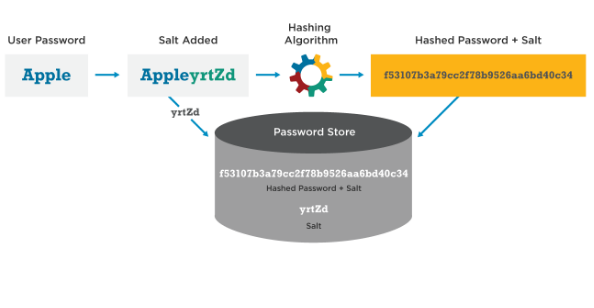
\includegraphics[scale=0.5]{images/prova.png}
        \caption{How salting works}
        \label{fig:salt}
    \end{figure}
    
    \FloatBarrier   
    
    As we can see salting is a good mitigation for the dictionary attacks.

    So we can see that the longer it takes to compute a digest, the longer a brute force attack will take. The work factor is the number of iterations of the hashing algorithm that are performed for each password, its purpose it's to make calculating the hash more computationally expensive. It's good to choice a balance between security and performance (general rule is that calculating a digest should take less than a second).

    Said that the risk of phishing remain (and with this the riks of get the password stolen).
    
    \subsection{Extension of password based authentication}
    We can extend the concept of passwords utilizing the multi factor authentication that can be performed by
    \begin{itemize}
        \item knowledge, something only the user knows (personal id number)
        \item ownership, something only the user possesses (token, smart card, phone)
        \item inherence, something the user is (biometrics)
    \end{itemize}
    The multi factor authentication is the combination of a password and another thing to perform the authentication (it can be also more than one another thing). The most common one is the 2FA (two factor authenticator), performed with a password and a OTP (one time password). Or a more common could be when you go to the ATM you insert the card and digit a PIN in order to use the services.
    
    \myparagraph{Time based One Time Password}
    OPT that has a deadline, they have two parameters the $T_0$ that is the Unix time from which start counting time steps, $T_x$ interval which will be used to calculate the value of the counter. Authenticator and authenticatee compute the TOTP value then the authenticator checks if the TOTP value supplied by the authenticated matches the locally-generated TOTP value. The weakness is that OTP values can be phished just as passwords can and replayed, another thing is that if the shared secret is no more secret an attacker could generate new valid TOTP.
    \begin{figure}[h!]
        \centering
        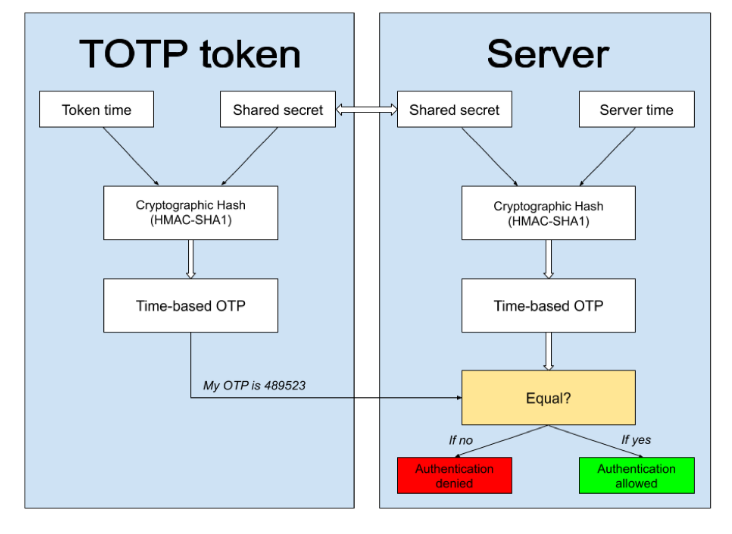
\includegraphics[scale=0.35]{images/TOTP.png}
        \caption{A TOTP communication}
        \label{fig:TOTP}
    \end{figure}
    
    \FloatBarrier   
    
    \myparagraph{Challenge Response Protocols}
    In CRP encryption convers the original representation of the information (\textbf{plaintext}) into an alternative form (ciphertext). Only authorized parties can decipher a ciphertext back to plaintext and access the original information. Encryption denies the intelligible content to a would-be interceptor.
    
    It's a mitigation for MITM attacks, since challenge changes at every connection and the password in clear doesn't leave the client, the MITM cannot reuse previously intercepted hashed password.
    
    \begin{figure}[h!]
        \centering
        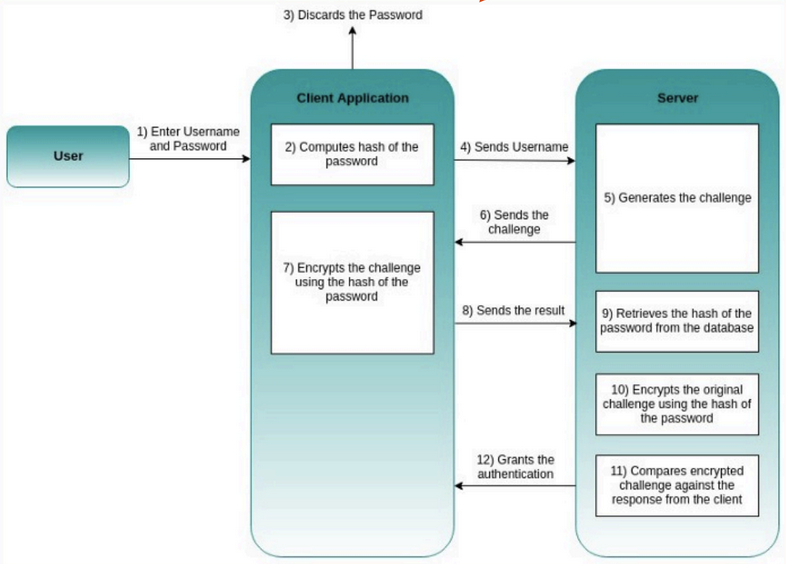
\includegraphics[scale=0.4]{images/CRP.png}
        \caption{CRP communication}
        \label{fig:CRP}
    \end{figure}
    
    \FloatBarrier   
    
    \myparagraph{PSD2}
    PSD2 is a solution to remove the TOTP hardware token, this because in the past they where hacked and they spoofed all the users. Chinese attackers spoofed Lockheed Martin staff-Sole plans for F-35 fighter jet. PSD2 idea is to include in the challenge the data that are unique to the particular transaction such as destination of transaction, amount of transaction ecc. But this is not enoungh, need to add random data.
    \\\\
    We can also use \textbf{smartphones} as part of MFA, no additional token are required, dinamically generated passcodes are safer. It has it's disadvantages too, a mobile phone is not always available, the mobile connection is not always available, there are sim cloners, text message could be stolen.
    \\\\
    \myparagraph{Assurance level NIST}
    \begin{enumerate}
        \item Provides some assurance that the claimant controls the authenticator, require at least a \textbf{single factor authentication.}
        \item Provides high confidence that the claimant controls authenicators, \textbf{two different authentication factor} are required.
        \item Provides very high confidence that the claimant controls the authenticator, authentication based on \textbf{proof of possession of a key} through a cryptographic protocol.
    \end{enumerate}
    
    Unfortunately even MFA procedures can be vulnerable to phishing attacks, example MFA fatigue attacks (flooding a user with push notification in the hope that will accept one).

    Phishing in general can be solved avoiding password!
    
    \myparagraph{FIDO}
    The main idea of fido is avoiding passwords, Google reported that it has not had any of it's 85000+ employees successfully phished on their work-related accounts since early 2017 when they started using physical security keys in place of passwords and one-time code.
    
    A security key implements a form of multi-factor authentication known as \textbf{Universal 2nd Factor (U2F)}, which allows the user to complete the login process simoly by inserting the USB device and pressing a button on it. Web Authentication API (\textbf{WebAuthn}) is a standard that eliminates the need for users to constantly type in their passwords and instead uses \textbf{Public key cryptography in combination with a challenge response protocol.} This avoid the possibility of phishing and MITM.
    
    FIDO requires an initial registration step: in cases where the user device supports multiple forms of authentication the user is asked to choose a FIDO compliant authenticator from the option available. The user then unlocks the FIDO authenticator using whatever mechanism is built into the authenticator, once is unlocked the user's device creates a new and unique public/private cryptographic key pair that will be used for authenticating access (\textbf{public one} is sent on the online server and associated with user account, the \textbf{private} and the other sensitive data remain on the local device and never leave it). Authentication requires the client device to prove possession of the private key by successfully respond to a cryptographic challenge. Private key can only be used after successfully authenticating using the registered authenticator, the device then uses the user account identifier provided by the service to select the correct key and cryptographically sign the service's challenge. Finally signed challenge is sent back to the service which verifies it and log in the user.
    
    \subsubsection{Outsourcing Authenticator}
    National digital identity infrastructures sponsored by many member states in europe obtained different level of success because of the not always clear business models for identity providers (an example of this is the Sistema Pubblico di Identità Digitale (SPID) in Italy). The problem is that securing all the phases of the identity management lifecycle is far from being trivial, organizations lack resources to devote ton security and need to focus on their core business. A solution could be to delegate the authentication to a trusted third party identity provider. Another example are the Single Sign On \textbf{(SSO)} like login with google or facebook ecc. This technique has lot of pros but a very big con: only one password to compose, if we use SSO+MFA we can improve a lot our security.
    Also it's a single point of failoure so needs to put more effort on the security part
    %--LECTURE PAGE 41--%
\section{Cryptography}
    \subsection{Introduction to Cryptography}
    \textbf{Cryptography} is the science and study of secret writing, \textbf{cryptoanalysis} is the science and the study of methods of breaking ciphers, \textbf{Cryptology} is cryptography and cryptoanalysis. Today cryptography is the study of mathematical techniques related to aspects of information security such as:
    \begin{itemize}
        \item \textbf{Confidentiality}: encryption algorithms hide the content of messages
        \item data \textbf{Integrity}: integrity check functions provide the means to detect whether a document has been changed
        \item entity authentication 
        \item data origin authentication: message authentication codes or digital signature algorithms provide the means to verify the source and integrity of a message
    \end{itemize}
    Cryptography is a security mechanism that includes a set of techniques for scrambling or disguising data so that is available only to someone who can restore the data to its original form. It provides a string economical basis for offering data security as a security service.
    
    \myparagraph{Cryptosystem}
    A cryptosystem is a 5-tuple (E,D,M,K,C) where
    \begin{itemize}
        \item \textbf{E} is an \textit{encryption} algorithm
        \item \textbf{D} is a \textit{decryption} algorithm
        \item \textbf{M} is the set of \textit{plaintexts}
        \item \textbf{K} is the set of \textit{keys} 
        \item \textbf{C} is the set of \textit{ciphertexts}
    \end{itemize}
    
    So $D(E(m,k),k)=m$, encryption and decryption keys are not necessarily the same (simmetric or asimmetric cryptography).
    
    \textbf{Kerckhoffs principle}: do not rely on the secrecy of algorithms, the key should be the only secret that needs protection
    
    \myparagraph{About Keys}
    A key is an input to a cryptographic algorithm used to obtain confidentiality, integrity and authenticity or other property over some data, security depends on keeping the key secret.
    
    %PAGE 12%

\end{document}
